\chapter{Functionalities}
\section{Entities}
We decided to offer the following entities which are the most important and common ones, which can be defined by the user of our software in XML:

\begin{itemize}
	\item{\textbf{Room}: a player can only be in one room at times. The room can be called whatever the designer decides. (for instance, desert, forest, dungeon)}
	\item{\textbf{Player}: the player in the world}
	\item{\textbf{Item}: an item which can be collected, used or equiped by the player.}
	\item{\textbf{Creature}: A creature can be allied, neutral or be your enemy. Additionally, creatures can hold items. Creatures may drop these items if they get killed.}
	\item{\textbf{Door}: A door simply is a connection between two rooms. Each door can have a guard which avoids passing.}
\end{itemize}

Our software should provide an interface for the user to create the content from above in XML, by defining first all existing entities and then creating the world (rooms and fill them with content).

\section{World design}

The world is divided into rooms. These rooms can be visited by the player. For some rooms he may need permission. In that case, he has to fit some requirements. These requirements (or guards) can be set in XML as well. Let us have a look at a simple world:

\begin{figure}[hb]
  \centering
  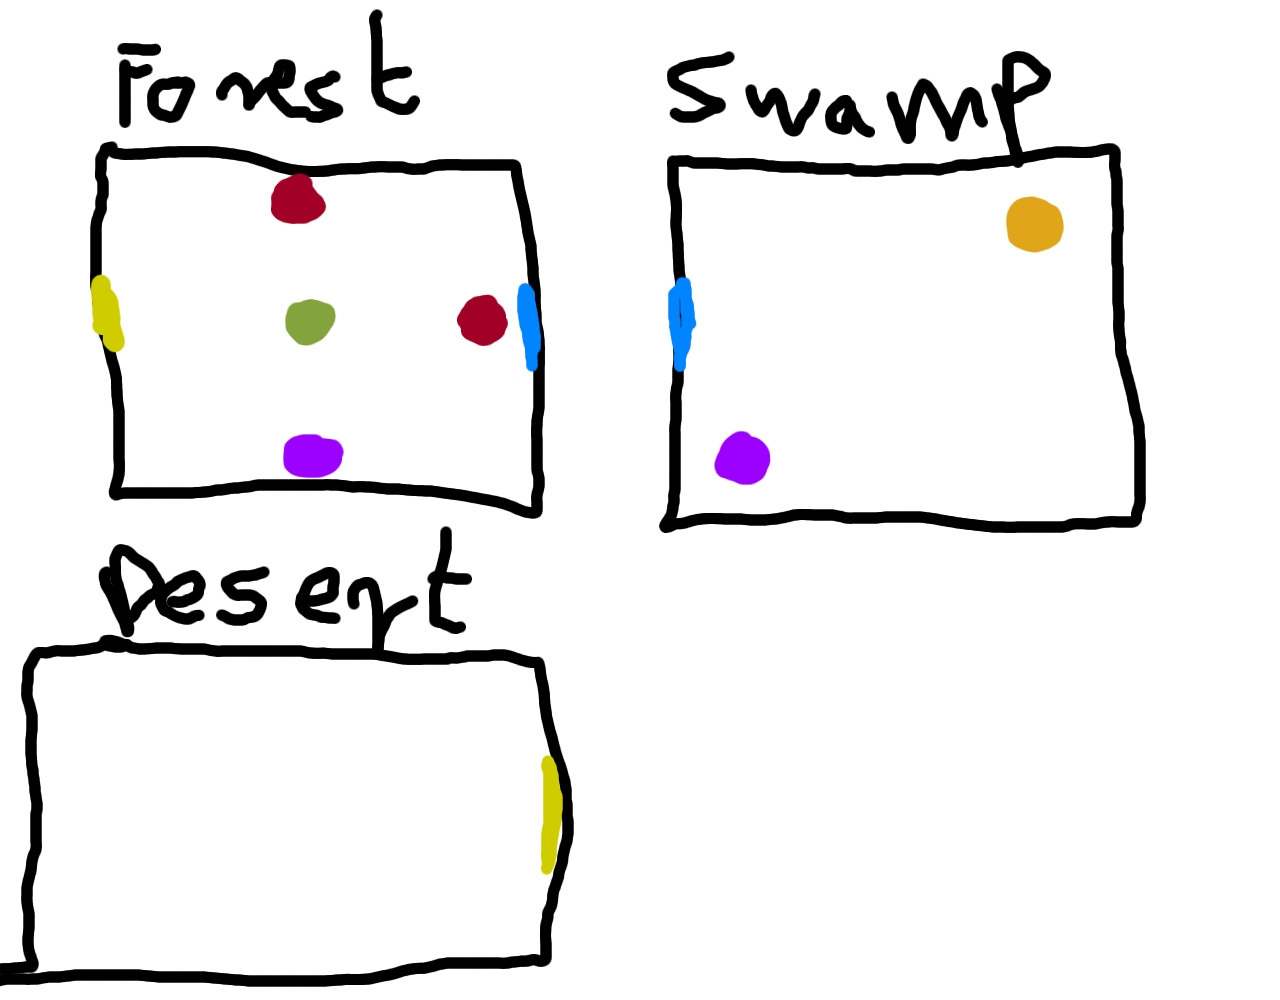
\includegraphics[width=4in]{../demo/demo.jpg}
  \caption{Each room is divided into 9 or more parts.}
\end{figure}

We want to create a simple world design where each room can have 9 or more parts. On each part can only be one game object at one time. It's also possible to move the player in a room or to pass doors due to enter other rooms. It is also possible to put game objects in each room. As you can see in the image, the green point is the player, the red ones are enemies, the yellow point is a neutral creature and the violet points are items, laying on the ground.

\section{Commands}
The game offers different commands for the player to interact with the game. These are the way the player controls his character in the game and how the game is played.
EPIC offers the following already fully implemented commands:
\begin{itemize}
\item Attack - Attacks a creature standing next to the player, also gets hit back by the creature.
\item Drop - Used to drop items to the ground.
\item Equip - Used to equip items from inventory.
\item Use - Used to use item from inventory. (Usable Items are not yet supported.)
\item Take - Used to pickup items from the world to the inventory
\end{itemize}

\section{Parsing}

We created an XML parsing part for \textbf{EPIC} which takes a single XML file that contains definitions of the different entities like player,creatures, items, rooms and doors. The whole game is inside the \textbf{adventure} tag and can be easly written. Each entities offers optional attributes to customize them in different ways.  Items and creatures for example can have different stats which are used when fighting.